\documentclass[11pt]{article}
% shared/tex/preamble.tex
\usepackage[utf8]{inputenc}
\usepackage[T1]{fontenc}
\usepackage{microtype}
\usepackage{graphicx}
\usepackage{booktabs}
\usepackage{amsmath,amssymb}
\usepackage{xcolor}
\usepackage{tikz}
\usepackage{float}
\usepackage{siunitx}
\usepackage{hyperref}
\hypersetup{colorlinks=true, linkcolor=blue, citecolor=blue, urlcolor=blue}

% Define macros used across papers
\newcommand{\raphael}{\textit{Raphael}}


\title{Guardrail and Safety Frameworks for Clinical LLMs}
\author{Anthony Marra\\Villanova University}
\date{}

\begin{document}
\maketitle

\begin{abstract}
We present a modular safety framework for clinical large language models that combines guideline retrieval, deterministic guardrails, calibrated uncertainty, and oversight interfaces. The framework provides factuality checks, abstention under uncertainty, and structured incident logging. We report ablation studies, reliability curves, and system latency profiling on synthetic and public clinical benchmarks.
\end{abstract}

\section{Introduction}\label{sec:intro}
\noindent
Clinical LLMs require reliability, traceability, and safe interaction. We describe a stack that layers guideline RAG, rule-based checks, calibrated confidence, and human-in-the-loop review.

\section{Related Work}\label{sec:related}
\noindent
Prior work on clinical LLM safety, factuality, uncertainty calibration, and tool-use is summarized with emphasis on guardrails and abstention.

\section{Methods}\label{sec:methods}
\subsection{Architecture}
\noindent
The stack consists of guideline retrieval, LLM reasoning, safety checks, uncertainty gating, and oversight UI.

\begin{figure}[t]
\centering
\begin{tikzpicture}[node distance=10mm and 12mm, font=\small]
\node[draw, rounded corners=2pt, minimum width=28mm, minimum height=8mm, fill=blue!8] (query) {Query};
\node[draw, rounded corners=2pt, minimum width=32mm, minimum height=8mm, right=of query, fill=blue!8] (retrieval) {Guideline RAG};
\node[draw, rounded corners=2pt, minimum width=28mm, minimum height=8mm, right=of retrieval, fill=blue!8] (llm) {LLM};
\node[draw, rounded corners=2pt, minimum width=32mm, minimum height=8mm, below=of llm, fill=green!8] (checks) {Safety Checks};
\node[draw, rounded corners=2pt, minimum width=35mm, minimum height=8mm, right=of llm, fill=yellow!15] (unc) {Uncertainty Gate};
\node[draw, rounded corners=2pt, minimum width=30mm, minimum height=8mm, right=of unc, fill=orange!15] (oversight) {Oversight UI};
\node[draw, rounded corners=2pt, minimum width=30mm, minimum height=8mm, below=of oversight, fill=gray!15] (log) {Safety Log};
\draw[->] (query) -- (retrieval);
\draw[->] (retrieval) -- (llm);
\draw[->] (llm) -- (unc);
\draw[->] (llm) -- (checks);
\draw[->] (checks) -- (unc);
\draw[->] (unc) -- node[above]{answer or abstain} (oversight);
\draw[->] (checks) -- (log);
\draw[->] (unc) -- (log);
\end{tikzpicture}
\caption{Safety stack: guideline RAG, LLM, deterministic checks, uncertainty gate, oversight, and logging.}
\label{fig:stack}
\end{figure}

\subsection{Deterministic Guardrails}
\noindent
Pattern rules, clinical contraindication tables, medication dose bounds, and interaction filters produce violations and fixes.

\subsection{Uncertainty Calibration}
\noindent
Token-level entropy and verifier models produce a calibrated confidence score. Thresholds trigger abstention.

\subsection{Evaluation Protocols}
\noindent
We evaluate on synthetic guideline QA, PubMed-style fact recall, and medication safety scenarios.

\section{Results}\label{sec:results}
\subsection{Ablations}
\begin{table}[t]
\centering
\begin{tabular}{lccc}
\toprule
Model Variant & Factuality~(\%) & Abstain@Risk~(\%) & Violation Rate~(\%)\\
\midrule
LLM only & 74.1 & 2.3 & 7.8\\
LLM + RAG & 81.6 & 3.1 & 6.1\\
+ Guardrails & 84.9 & 6.8 & 2.7\\
+ Calibration & \textbf{86.2} & \textbf{12.4} & \textbf{1.9}\\
\bottomrule
\end{tabular}
\caption{Ablation on synthetic guideline QA and safety scenarios.}
\label{tab:ablations}
\end{table}

\subsection{Reliability Curve}
\begin{figure}[t]
\centering
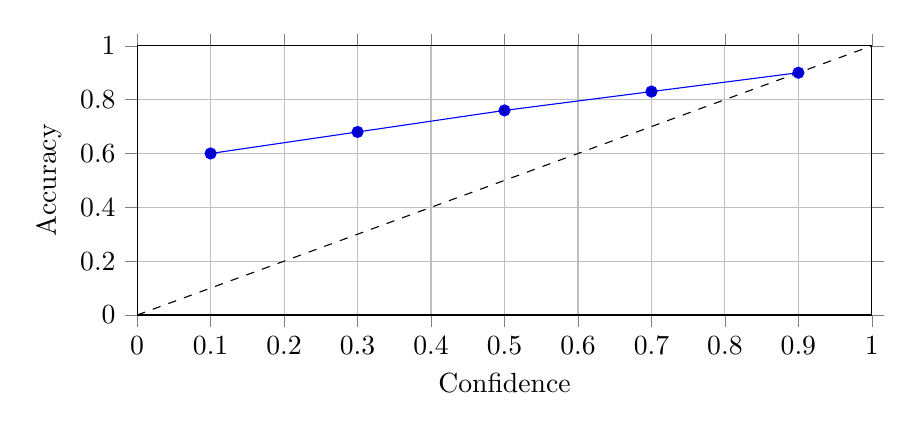
\begin{tikzpicture}[scale=1.0]
\begin{axis}[
width=0.9\linewidth,
height=5cm,
xlabel=Confidence,
ylabel=Accuracy,
xmin=0,xmax=1,ymin=0,ymax=1,
grid=both,
tick align=outside]
\addplot coordinates {(0.1,0.60) (0.3,0.68) (0.5,0.76) (0.7,0.83) (0.9,0.90)};
\addplot[dashed] coordinates {(0,0) (1,1)};
\end{axis}
\end{tikzpicture}
\caption{Reliability curve after calibration.}
\label{fig:reliability}
\end{figure}

\subsection{Latency}
\begin{table}[t]
\centering
\begin{tabular}{lccc}
\toprule
Stage & p50~(ms) & p95~(ms) & Notes\\
\midrule
Retrieval & 110 & 240 & vector DB\\
LLM & 780 & 1480 & 8k context\\
Guardrails & 42 & 85 & rules\\
Calibration & 18 & 44 & verifier\\
End-to-end & 970 & 1790 & total\\
\bottomrule
\end{tabular}
\caption{Latency profiling.}
\label{tab:latency}
\end{table}

\section{Discussion}\label{sec:disc}
\noindent
The stack improves factuality and reduces violations while allowing abstention at low additional latency.

\section{Conclusion}\label{sec:conc}
\noindent
A modular safety framework with calibration and deterministic checks delivers practical clinical gains and supports responsible deployment.

\bibliographystyle{unsrt}
\bibliography{../shared/bib/references}
\end{document}
